\documentclass[
	% -- opções da classe memoir --
	12pt,				% tamanho da fonte
	openright,			% capítulos começam em pág ímpar (insere página vazia caso preciso)
	oneside,			    % para impressão em recto e verso usar two side (Oposto a oneside)
	a4paper,				% tamanho do papel. 
	% -- opções da classe abntex2 --
	%chapter=TITLE,		% títulos de capítulos convertidos em letras maiúsculas
	%section=TITLE,		% títulos de seções convertidos em letras maiúsculas
	%subsection=TITLE,	% títulos de subseções convertidos em letras maiúsculas
	%subsubsection=TITLE,% títulos de subsubseções convertidos em letras maiúsculas
	% -- opções do pacote babel --
	english,			% idioma adicional para hifenização
	french,			% idioma adicional para hifenização
	spanish,			% idioma adicional para hifenização
	brazil			% o último idioma é o principal do documento
	]{abntex2}

% ---
% Pacotes básicos 
% ---
\usepackage{array}
\usepackage{lmodern}			% Usa a fonte Latin Modern			
\usepackage[T1]{fontenc}		% Selecao de codigos de fonte.
\usepackage[utf8]{inputenc}	% Codificacao do documento (conversão automática dos acentos)
\usepackage{indentfirst}		% Indenta o primeiro parágrafo de cada seção.
\usepackage{color}			% Controle das cores
\usepackage{graphicx}		% Inclusão de gráficos
\usepackage{microtype} 	
% para melhorias de justificação
% ---
		
% ---
% Pacotes adicionais, usados apenas no âmbito do Modelo Canônico do abnteX2
% ---
%\usepackage{lipsum}				% para geração de dummy text
% ---

% ---
% Pacotes de citações
% ---
\usepackage[brazilian,hyperpageref]{backref}	 % Paginas com as citações na bibl
\usepackage[alf]{abntex2cite}	% Citações padrão ABNT

% --- 
% CONFIGURAÇÕES DE PACOTES
% --- 

% ---
% Configurações do pacote backref
% Usado sem a opção hyperpageref de backref
% \renewcommand{\backrefpagesname}{Citado na(s) página(s):~}
% Texto padrão antes do número das páginas
%\renewcommand{\backref}{}
% Define os textos da citação
%\renewcommand*{\backrefalt}[4]{
%	\ifcase #1 %
%		Nenhuma citação no texto.%
%	\or
%		Citado na página #2.%
%	\else
%		Citado #1 vezes nas páginas #2.%
%	\fi}%
% ---

% ---
% Informações de dados para CAPA e FOLHA DE ROSTO
% ---
\titulo{Aplicação de LLM com RAG para consulta de processos ambientais}
\autor{Cesar Hideki Imai \\ David Varão Lima Bentes Pessoa \\ João Victor Dallapé Madeira}
\local{São Paulo}
\data{2022}
\orientador{Lucas Cerqueira Figueiredo}

\instituicao{%
  Universidade Presbiteriana Mackenzie
  \par
  Faculdade de Computação e Informática}
\tipotrabalho{Tipo do Trabalho (TCC)}
% O preambulo deve conter o tipo do trabalho, o objetivo, 
% o nome da instituição e a área de concentração 
\preambulo{Documentação Inicial do Trabalho de Conclusão de Curso SamsAI para a disciplina de Laboratório de Engenharia de Software }
% ---


% ---
% Configurações de aparência do PDF final

% alterando o aspecto da cor azul
\definecolor{blue}{RGB}{41,5,195}

% informações do PDF
\makeatletter
\hypersetup{
     	%pagebackref=true,
		pdftitle={\@title}, 
		pdfauthor={\@author},
    		pdfsubject={\imprimirpreambulo},
	    pdfcreator={LaTeX with abnTeX2},
		pdfkeywords={abnt}{latex}{abntex}{abntex2}{trabalho acadêmico}, 
		colorlinks=true,       	% false: boxed links; true: colored links
    		linkcolor=blue,          % color of internal links
    		citecolor=blue,        	% color of links to bibliography
    		filecolor=magenta,      	% color of file links
		urlcolor=blue,
		bookmarksdepth=4
}
\makeatother
% --- 

% ---
% Posiciona figuras e tabelas no topo da página quando adicionadas sozinhas
% em um página em branco. Ver https://github.com/abntex/abntex2/issues/170
\makeatletter
\setlength{\@fptop}{5pt} % Set distance from top of page to first float
\makeatother
% ---

% ---
% Possibilita criação de Quadros e Lista de quadros.
% Ver https://github.com/abntex/abntex2/issues/176
%
\newcommand{\quadroname}{Quadro}
\newcommand{\listofquadrosname}{Lista de quadros}

\newfloat[chapter]{quadro}{loq}{\quadroname}
\newlistof{listofquadros}{loq}{\listofquadrosname}
\newlistentry{quadro}{loq}{0}

% configurações para atender às regras da ABNT
\setfloatadjustment{quadro}{\centering}
\counterwithout{quadro}{chapter}
\renewcommand{\cftquadroname}{\quadroname\space} 
\renewcommand*{\cftquadroaftersnum}{\hfill--\hfill}

\setfloatlocations{quadro}{hbtp} % Ver https://github.com/abntex/abntex2/issues/176
% ---

% --- 
% Espaçamentos entre linhas e parágrafos 
% --- 

% O tamanho do parágrafo é dado por:
\setlength{\parindent}{1.3cm}

% Controle do espaçamento entre um parágrafo e outro:
\setlength{\parskip}{0.2cm}  % tente também \onelineskip

% ---
% compila o indice
% ---
\makeindex
% ---

% ----
% Início do documento
% ----
\begin{document}

% Seleciona o idioma do documento (conforme pacotes do babel)
%\selectlanguage{english}
\selectlanguage{brazil}

% Retira espaço extra obsoleto entre as frases.
\frenchspacing 

% ----------------------------------------------------------
% ELEMENTOS PRÉ-TEXTUAIS
% ----------------------------------------------------------
% \pretextual

% ---
% Capa
% ---
\imprimircapa
% ---

% ---
% Folha de rosto
% (o * indica que haverá a ficha bibliográfica)
% ---
\imprimirfolhaderosto*
% ---

% ---
% Inserir a ficha bibliografica
% ---

% Isto é um exemplo de Ficha Catalográfica, ou ``Dados internacionais de
% catalogação-na-publicação''. Você pode utilizar este modelo como referência. 
% Porém, provavelmente a biblioteca da sua universidade lhe fornecerá um PDF
% com a ficha catalográfica definitiva após a defesa do trabalho. Quando estiver
% com o documento, salve-o como PDF no diretório do seu projeto e substitua todo
% o conteúdo de implementação deste arquivo pelo comando abaixo:
%
% \begin{fichacatalografica}
%     \includepdf{fig_ficha_catalografica.pdf}
% \end{fichacatalografica}

\begin{fichacatalografica}
	\sffamily
	\vspace*{\fill}					% Posição vertical
	\begin{center}					% Minipage Centralizado
	\fbox{\begin{minipage}[c][8cm]{13.5cm}		% Largura
	\small
	\imprimirautor
	%Sobrenome, Nome do autor
	
	\hspace{0.5cm} \imprimirtitulo  / \imprimirautor. --
	\imprimirlocal, \imprimirdata-
	
	\hspace{0.5cm} \thelastpage p. : il. (algumas color.) ; 30 cm.\\
	
	\hspace{0.5cm} \imprimirorientadorRotulo~\imprimirorientador\\
	
	\hspace{0.5cm}
	\parbox[t]{\textwidth}{\imprimirtipotrabalho~--~\imprimirinstituicao,
	\imprimirdata.}\\
	
	\hspace{0.5cm}
		1. Palavra-chave1: Large Language Model
		2. Palavra-chave2: Retrieval Augmented Generation
		2. Palavra-chave3: Direito ambiental
		I. Orientador: Lucas Cerqueira Figueiredo
		II. Universidade Presbiteriana Mackenzie.
		III. Faculdade de Computação e Informática.
		IV. Aplicação de LLM com RAG para consulta de processos ambientais
	\end{minipage}}
	\end{center}
\end{fichacatalografica}
% ---

% ---
% Inserir errata
% ---
%\begin{errata}
%Elemento opcional da \citeonline[4.2.1.2]{NBR14724:2011}. Exemplo:
%
%\vspace{\onelineskip}
%
%FERRIGNO, C. R. A. \textbf{Tratamento de neoplasias ósseas apendiculares com
%reimplantação de enxerto ósseo autólogo autoclavado associado ao plasma
%rico em plaquetas}: estudo crítico na cirurgia de preservação de membro em
%cães. 2011. 128 f. Tese (Livre-Docência) - Faculdade de Medicina Veterinária e
%Zootecnia, Universidade de São Paulo, São Paulo, 2011.
%
%\begin{table}[htb]
%\center
%\footnotesize
%\begin{tabular}{|p{1.4cm}|p{1cm}|p{3cm}|p{3cm}|}
%  \hline
%   \textbf{Folha} & \textbf{Linha}  & \textbf{Onde se lê}  & \textbf{Leia-se}  \\
%    \hline
%    1 & 10 & auto-conclavo & autoconclavo\\
%   \hline
%\end{tabular}
%\end{table}
%
%\end{errata}
% ---

% ---
% Inserir folha de aprovação
% ---

% Isto é um exemplo de Folha de aprovação, elemento obrigatório da NBR
% 14724/2011 (seção 4.2.1.3). Você pode utilizar este modelo até a aprovação
% do trabalho. Após isso, substitua todo o conteúdo deste arquivo por uma
% imagem da página assinada pela banca com o comando abaixo:
%
% \begin{folhadeaprovacao}
% \includepdf{folhadeaprovacao_final.pdf}
% \end{folhadeaprovacao}
%
%\begin{folhadeaprovacao}
%
%  \begin{center}
%    {\ABNTEXchapterfont\large\imprimirautor}
%
%    \vspace*{\fill}\vspace*{\fill}
%    \begin{center}
%      \ABNTEXchapterfont\bfseries\Large\imprimirtitulo
%    \end{center}
%    \vspace*{\fill}
%    
%    \hspace{.45\textwidth}
%    \begin{minipage}{.5\textwidth}
%        \imprimirpreambulo
%    \end{minipage}%
%    \vspace*{\fill}
%   \end{center}
%        
%   Trabalho aprovado. \imprimirlocal, 24 de novembro de 2012:
%
%   \assinatura{\textbf{\imprimirorientador} \\ Orientador} 
%   \assinatura{\textbf{Professor} \\ Convidado 1}
%   \assinatura{\textbf{Professor} \\ Convidado 2}
%   %\assinatura{\textbf{Professor} \\ Convidado 3}
%   %\assinatura{\textbf{Professor} \\ Convidado 4}
%      
%   \begin{center}
%    \vspace*{0.5cm}
%    {\large\imprimirlocal}
%    \par
%    {\large\imprimirdata}
%    \vspace*{1cm}
%  \end{center}
%  
%\end{folhadeaprovacao}
% ---

% ---
% Dedicatória
% ---
%\begin{dedicatoria}
%   \vspace*{\fill}
%   \centering
%   \noindent
%   \textit{ Este trabalho é dedicado às crianças adultas que,\\
%   quando pequenas, sonharam em se tornar cientistas.} \vspace*{\fill}
%\end{dedicatoria}
% ---

% ---
% Agradecimentos
% ---
%\begin{agradecimentos}
%Os agradecimentos principais são direcionados à Gerald Weber, Miguel Frasson,
%Leslie H. Watter, Bruno Parente Lima, Flávio de Vasconcellos Corrêa, Otavio Real
%Salvador, Renato Machnievscz\footnote{Os nomes dos integrantes do primeiro
%projeto abn\TeX\ foram extraídos de
%\url{http://codigolivre.org.br/projects/abntex/}} e todos aqueles que
%contribuíram para que a produção de trabalhos acadêmicos conforme
%as normas ABNT com \LaTeX\ fosse possível.
%
%Agradecimentos especiais são direcionados ao Centro de Pesquisa em Arquitetura
%da Informação\footnote{\url{http://www.cpai.unb.br/}} da Universidade de
%Brasília (CPAI), ao grupo de usuários
%\emph{latex-br}\footnote{\url{http://groups.google.com/group/latex-br}} e aos
%novos voluntários do grupo
%\emph{\abnTeX}\footnote{\url{http://groups.google.com/group/abntex2} e
%\url{http://www.abntex.net.br/}}~que contribuíram e que ainda
%contribuirão para a evolução do \abnTeX.
%
%\end{agradecimentos}
% ---

% ---
% Epígrafe
% ---
%\begin{epigrafe}
%    \vspace*{\fill}
%	\begin{flushright}
%		\textit{``Não vos amoldeis às estruturas deste mundo, \\
%		mas transformai-vos pela renovação da mente, \\
%		a fim de distinguir qual é a vontade de Deus: \\
%		o que é bom, o que Lhe é agradável, o que é perfeito.\\
%		(Bíblia Sagrada, Romanos 12, 2)}
%	\end{flushright}
%\end{epigrafe}
% ---

% ---
% RESUMOS
% ---

% resumo em português
%\setlength{\absparsep}{18pt} % ajusta o espaçamento dos parágrafos do resumo
%\begin{resumo}
% Segundo a \citeonline[3.1-3.2]{NBR6028:2003}, o resumo deve ressaltar o
% objetivo, o método, os resultados e as conclusões do documento. A ordem e a extensão
% destes itens dependem do tipo de resumo (informativo ou indicativo) e do
% tratamento que cada item recebe no documento original. O resumo deve ser
% precedido da referência do documento, com exceção do resumo inserido no
% próprio documento. (\ldots) As palavras-chave devem figurar logo abaixo do
% resumo, antecedidas da expressão Palavras-chave:, separadas entre si por
% ponto e finalizadas também por ponto.
%
% \textbf{Palavras-chave}: latex. abntex. editoração de texto.
%\end{resumo}
%
%% resumo em inglês
%\begin{resumo}[Abstract]
% \begin{otherlanguage*}{english}
%   This is the english abstract.
%
%   \vspace{\onelineskip}
% 
%   \noindent 
%   \textbf{Keywords}: latex. abntex. text editoration.
% \end{otherlanguage*}
%\end{resumo}
%
%% resumo em francês 
%\begin{resumo}[Résumé]
% \begin{otherlanguage*}{french}
%    Il s'agit d'un résumé en français.
% 
%   \textbf{Mots-clés}: latex. abntex. publication de textes.
% \end{otherlanguage*}
%\end{resumo}
%
%% resumo em espanhol
%\begin{resumo}[Resumen]
% \begin{otherlanguage*}{spanish}
%   Este es el resumen en español.
%  
%   \textbf{Palabras clave}: latex. abntex. publicación de textos.
% \end{otherlanguage*}
%\end{resumo}
% ---

% ---
% inserir lista de ilustrações
% ---
\newpage
\pdfbookmark[0]{\listfigurename}{lof}
\listoffigures*
\cleardoublepage
% ---

% ---
% inserir lista de quadros
% ---
\pdfbookmark[0]{\listofquadrosname}{loq}
\listofquadros*
\cleardoublepage
% ---

% ---
% inserir lista de tabelas
% ---
\pdfbookmark[0]{\listtablename}{lot}
\listoftables*
\cleardoublepage
% ---

% ---
% inserir lista de abreviaturas e siglas
% ---
\begin{siglas}
  \item[UC] Caso de Uso
  \item [LLM] Large Language Model
  \item [RAG] Retrieval Augmented Generation
\end{siglas}
% ---

% ---
% inserir o sumario
% ---
\pdfbookmark[0]{\contentsname}{toc}
\tableofcontents*
\cleardoublepage
% ---



% ----------------------------------------------------------
% ELEMENTOS TEXTUAIS
% ----------------------------------------------------------
\textual


\chapter{Introdução}
Em nosso país, o sistema judiciário desempenha um papel crucial para a sociedade: administrar a justiça. Sua função é garantir os direitos individuais, coletivos e sociais e resolver conflitos entre cidadãos, entidades e Estado. Porém, há dois grandes desafios a superar quando se trata da eficiência processual e da velocidade com que os casos são solucionados.

O Conselho Nacional de Justiça (CNJ) publicou recentemente o Relatório Justiça em Números 2024. O documento afirma que existem quase  84 milhões de processos tramitando no Brasil, que só aumentam a cada ano que passa. Sendo assim, o poder Judiciário acaba sendo sobrecarregado pelo enorme volume de processos.

Além disso, devido a enorme burocracia presente no poder Judiciário, os processos se tornam mais lentos, exigindo análises e pesquisas minuciosas por parte dos juízes e advogados.

Portanto, a ideia deste projeto é desenvolver uma aplicação  Large Language Model (LLM) com Retrieval Augmented Generation (RAG) capaz de unificar a origem de documentos jurídicos e gerar respostas baseadas nas informações dos documentos, que tenham proximidade com a informação desejada por meio de inteligência artificial. Dessa forma, seria possível tornar o procedimento de consulta e pesquisa de documentos mais ágil e menos exaustivo para os usuários "desafogando", assim, o poder Judiciário. Contudo, é importante destacar que este trabalho se limita à área do direito ambiental.



\chapter{Definição da Demanda}

\section{Descrição do projeto e definição dos usuários}

A fim de cumprir o objetivo deste projeto, será desenvolvida uma aplicação web, semelhante ao ChatGPT, que seja capaz de entregar ao usuário respostas contendo as informações de documentos judiciais necessários para o andamento de um processo (como legislações, acórdãos e súmulas) no âmbito do direito ambiental. Para diminuir as possíveis alucinações da Inteligência Artificial (IA), será aplicada a técnica RAG, em que se utilizará um banco de dados contendo estes documentos judiciais para que a IA o consulte. Sendo assim, os potenciais usuários de nossa aplicação são: estudantes de direito, juízes, desembargadores, procuradores e advogados.

\section{Etapas para a construção da aplicação e critérios}
\begin{enumerate}
  \item Adquirir um conjunto de documentos jurídicos para o teste;
  \item 
    \begin{enumerate}
    \item Deve ter documentos com temas ambientais;
    \item Deve conter acórdãos;
    \item Deve conter súmulas;
    \end{enumerate}
    
  \item Escolher um LLM treinado (Sabiá-3, ChatGPT);
  \item 
    \begin{enumerate}
    \item Deve ser priorizado o menor custo;
    \item Deve ter capacidade mínima de 4000 tokens por prompt;
    \end{enumerate}
  \item Estudar um dos frameworks (LlamaIndex ou Langchain) para aplicação RAG;
  \item Fazer a integração do LLM através do framework (por chave de API ou baixado localmente);
  \item 
    \begin{enumerate}
    \item Deve demorar no máximo 20 segundos para gerar a resposta;
    \end{enumerate}

  \item Fazer a integração da fonte externa (conjunto de documentos) através do framework;
  \item Integração com um banco de dados fornecido pela AWS;
  \item Testar o sistema;
  \item Construção da interface web da aplicação;
  \item Integração com a interface web;
  \item Testar o sistema com a interface.  
\end{enumerate}

\chapter{REQUISITOS DO PRODUTO}
Neste capítulo, são apresentados os requisitos que foram levantados. Separamos os requisitos em duas tabelas, na Tabela 1, os funcionais e, na Tabela 2, os não funcionais. Em cada uma delas, cada linha corresponde a um requisito, enquanto a coluna "ID" indica seu código de identificação, "Requisito" contém uma breve explicação do mesmo, "Tipo de requisito" classifica-o (funcional, usabilidade, software, desempenho, dados escalabilidade) e, por fim, a coluna  "Prioridade" exibe sua relevância. Os níveis de prioridade impostos são:
\begin{itemize}
  \item \textbf{Essencial:} é o requisito que o sistema não consegue operar em sua ausência; 
  \item \textbf{Importante:} é o requisitos que o sistema consegue funcionar em sua ausência, mas seu funcionamento fica comprometido;
  \item \textbf{Desejável:} é o requisito opcional, o sistema não é comprometido mesmo em sua ausência.
\end{itemize}


% TENTEI CENTRALIZAR, MAS NÃO DEU CERTO :( ODEIO O LATEX!!
%-------------------------- TABELA DE REQUISITOS FUNCIONAIS --------------------------------------------
\begin{table}[htb]
%\c
\ABNTEXfontereduzida
\caption[Requisitos funcionais]{Requisitos funcionais}
\label{tab-nivinv}
\hspace*{-1.4cm}
\begin{tabular}{|>{\centering\arraybackslash}m{1.2cm}|>{\centering\arraybackslash}m{10cm}|>{\centering\arraybackslash}m{2.25cm}|>{\centering\arraybackslash}m{2.2cm}|}
  \hline
   \textbf{ID} & \textbf{Requisitos funcionais}  & \textbf{Tipo de Requisito}  & \textbf{Prioridade}  \\
    \hline
    [RF01]& O sistema deve armazenar informações presentes em acórdãos para consulta.  & Funcional &
    Essencial  \\
    \hline
    [RF02] & O sistema deve armazenar informações presentes em súmulas para consulta. & Funcional  & Essencial \\
    \hline
    [RF03] & O sistema deve armazenar informações presentes em orientações jurisprudenciais para consulta. & Funcional & Essencial \\
    \hline
    [RF04] & O sistema deve atender palavras-chaves para a busca. & Funcional & Essencial \\
    \hline
    [RF05] & O sistema deve atender filtro por tipo de documento (legislação, acórdão, súmula, etc). & Funcional & Essencial \\
    \hline
    [RF06] & O sistema deve atender filtro por tribunal (STF, STJ, TJs, etc). & Funcional & Essencial \\
    \hline
    [RF07] & O sistema deve atender filtro por estado. & Funcional & Essencial \\
    \hline
    [RF08] & O sistema deve armazenar informações presentes em legislações para consulta & Funcional & Importante \\
    \hline
    [RF09] & O sistema deve armazenar informações presentes em sentenças para consulta.. & Funcional & Importante \\
    \hline
    [RF10] & O sistema deve armazenar informações presentes em decisões monocráticas para consulta. & Funcional & Importante \\
    \hline
    [RF11] & O sistema deve armazenar informações presentes em decisões interlocutórias para consulta. & Funcional & Importante \\
    \hline
    [RF12] & O sistema deve armazenar informações presentes em despachos para consulta. & Funcional & Importante \\
    \hline
    [RF13] & O sistema deve atender filtro por nome do relator & Funcional & Importante \\
    \hline
    [RF14] & O sistema deve atender filtro por tipo de processo (trabalhista, penal, etc). & Funcional & Importante \\
    \hline
    [RF15] & O sistema deve atender filtro por data. & Funcional & Importante \\
    \hline
    [RF16] & O sistema deve elaborar modelos de peças jurídicas. & Funcional & Importante \\
    \hline
    [RF17] & O sistema deve retornar a identificação dos documentos com suas ementas resumidas. & Funcional & Importante \\
    \hline
    [RF18] & O sistema deve retornar a descrição das legislações usadas numa decisão. & Funcional & Importante \\
    \hline
    [RF19] & O sistema deve resumir os argumentos de uma decisão. & Funcional & Importante \\
    \hline
    [RF20] & O sistema deve resumir a conclusão de uma decisão. & Funcional & Importante \\
    \hline
    [RF21] & O sistema deve auxiliar na interpretação de trechos de texto & Funcional & Importante \\
    \hline
    [RF22] & O usuário deve poder ajustar o tema da interface (tema claro ou escuro) & Funcional & Importante \\
    \hline
    [RF23] & O usuário deve poder fazer o download dos documentos recuperados. & Funcional & Importante \\
    \hline
    [RF24] & O usuário deve poder visualizar o histórico de conversas. & Funcional & Importante \\
    \hline
    [RF25] & O sistema deve retornar a identificação dos documentos com os trechos que tenham proximidade com a busca. & Funcional & Desejável \\
    \hline
    [RF26] & O sistema deve ter a opção dos usuários enviarem feedback (sugestões de melhorias e correções). & Funcional & Desejável \\
    \hline
    [RF27] & O sistema deve conter recursos text-to-speech (texto para fala) e speech-to-text (fala para texto). & Funcional & Desejável \\
    \hline
    [RF28] & O sistema deve ter versão mobile (acessível no celular). & Funcional & Desejável \\
    \hline
    [RF29] & O usuário deve poder visualizar o histórico de conversas. & Funcional & Desejável \\
    \hline
    [RF30] & O usuário deve poder apagar e arquivar conversas & Funcional & Desejável \\
    \hline
\end{tabular}
\legend{Fonte: Próprios autores}
\end{table}
%-------------------------- TABELA DE REQUISITOS FUNCIONAIS --------------------------------------------

%-------------------------- TABELA DE REQUISITOS NÃO FUNCIONAIS --------------------------------------------
\begin{table}[htb]
%\c
\ABNTEXfontereduzida
\caption[Requisitos não funcionais]{Requisitos não funcionais}
\label{tab-nivinv}
\hspace*{-1.7cm}
\begin{tabular}{|>{\centering\arraybackslash}m{1.2cm}|>{\centering\arraybackslash}m{10cm}|>{\centering\arraybackslash}m{2.25cm}|>{\centering\arraybackslash}m{2.2cm}|}
  \hline
   \textbf{ID} & \textbf{Requisitos não funcionais}  & \textbf{Tipo de Requisito}  & \textbf{Prioridade}  \\
    \hline
    [RNF01]& O sistema deve ser integrado com uma interface web simples com o prompt de entrada em destaque & Usabilidade &
    Essencial  \\
    \hline
    [RNF02] & O sistema deve ser compatível com diferentes navegadores web (Mozilla, Chrome, Opera, etc.) & Software & Essencial \\
    \hline
    [RFN03] & O sistema deve utilizar apenas os dados com proximidade igual ou maior a 50\% do texto de entrada e dar uma saída de “informações insuficientes” caso não tenha. & Dados & Essencial \\
    \hline
    [RNF04] & O sistema deve lidar com no mínimo 3 acessos simultâneos. & Escalabilidade & Essencial \\
    \hline
    [RNF05] & O sistema deve ser integrado com um serviço de banco de dados fornecido pela AWS para armazenar e consultar dados. & Dados & Essencial \\
    \hline
    [RNF06] & O sistema deve ser gerenciável para adição de novos dados de fontes externas. & Dados & Essencial \\
    \hline
    [RNF07] & O sistema deve ter login de contas para salvar as configurações e conversas. & Usabilidade & Essencial \\
    \hline
    [RNF08] & O código deve ser bem documentado, de modo a facilitar futuras atualizações e manutenção do sistema. & Software & Importante \\
    \hline
    [RNF09] & O sistema deve fazer uso de criptografia para proteger as conversas dos usuários. & Segurança & Importante \\
    \hline
    [RNF10] & O sistema deve ter um tempo de resposta de no máximo 20 segundos. & Usabilidade & Importante \\
    \hline
    [RNF11] & O sistema deve ser aprovado pelo PageSpeed Insights. & Desempenho & Importante \\
    \hline
    [RNF12] & O sistema deve ser responsivo, ou seja, que se adapta automaticamente ao dispositivo do utilizador, seja um desktop, tablet ou telemóvel. & Usabilidade & Importante \\
    \hline
    [RNF13] & O sistema deve evitar cores relacionadas ao daltonismo. & Usabilidade & Desejável \\
    \hline
\end{tabular}
\legend{Fonte: Próprios autores}
\end{table}
%-------------------------- TABELA DE REQUISITOS NÃO FUNCIONAIS --------------------------------------------

%-------------------------- FAZER A TABELA --------------------------------------------
\chapter{WIREFRAMES} %ADICIONAR WIREFRAMES
Com base nos requisitos funcionais descritos no capítulo 2, elaboramos protótipos de baixa fidelidade (wireframes) das telas da aplicação.

\section{Tela de Login}
Assim que o usuário entrar no site, ele deverá efetuar o login com seu email de acesso e respectiva senha.

\begin{figure}[h]
    \centering
    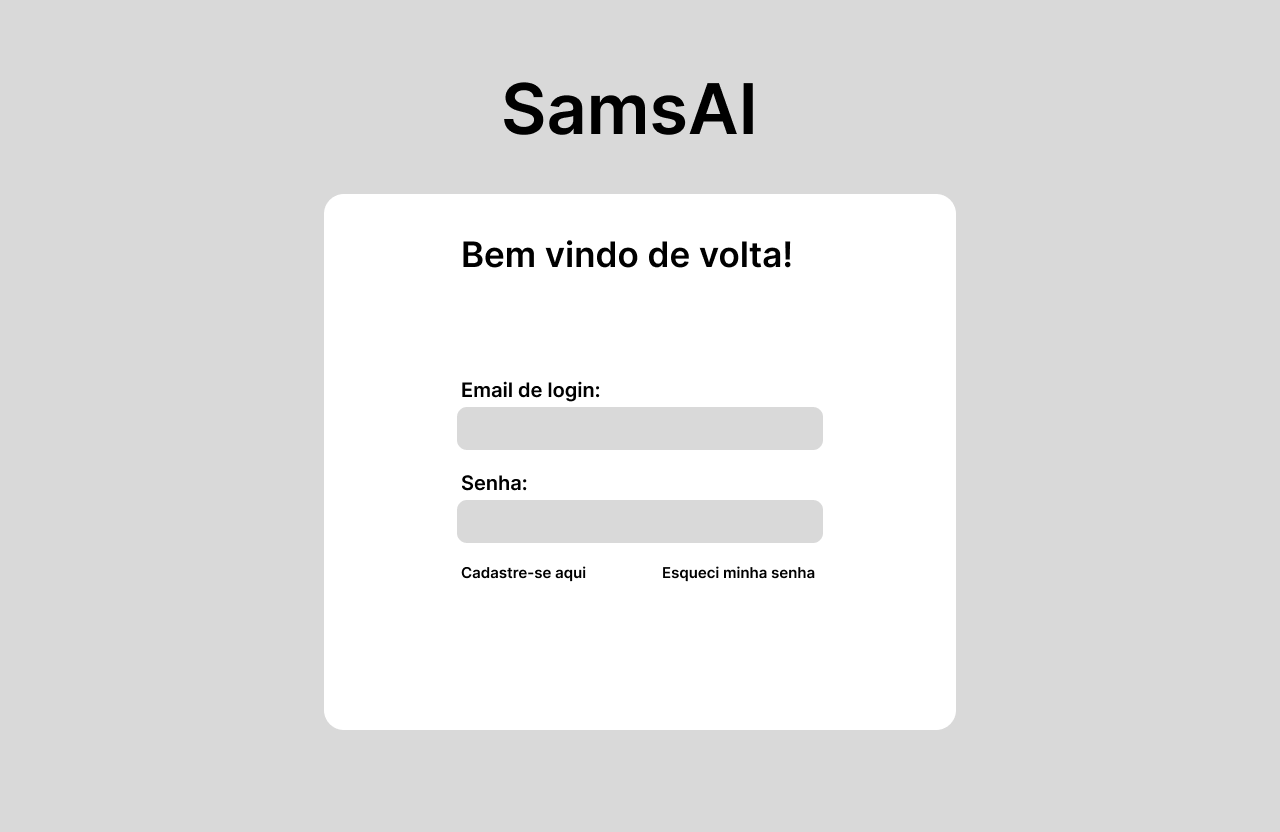
\includegraphics[width=0.8\linewidth]{Tela de Login.png}
    \caption{Tela de Login}
    \label{fig:enter-label}
\end{figure}

\section{Tela inicial (iniciar conversa)}
Após efetuar o login com sucesso, ele é convidado a iniciar uma nova conversa com a IA através de um chat, em que o usuário pode interagir escrevendo uma mensagem na caixa de entrada de texto no canto inferior da tela. Para enviar, ele deve clicar no ícone de enviar mensagem. 

Além disso, é também possível fazer upload de arquivos e mandá-los clicando no "clips" à esquerda. Também, ao invés de escrever, pode-se falar por voz a mensagem a ser enviada clicando no microfone à direita.

\begin{figure}[h]
    \centering
    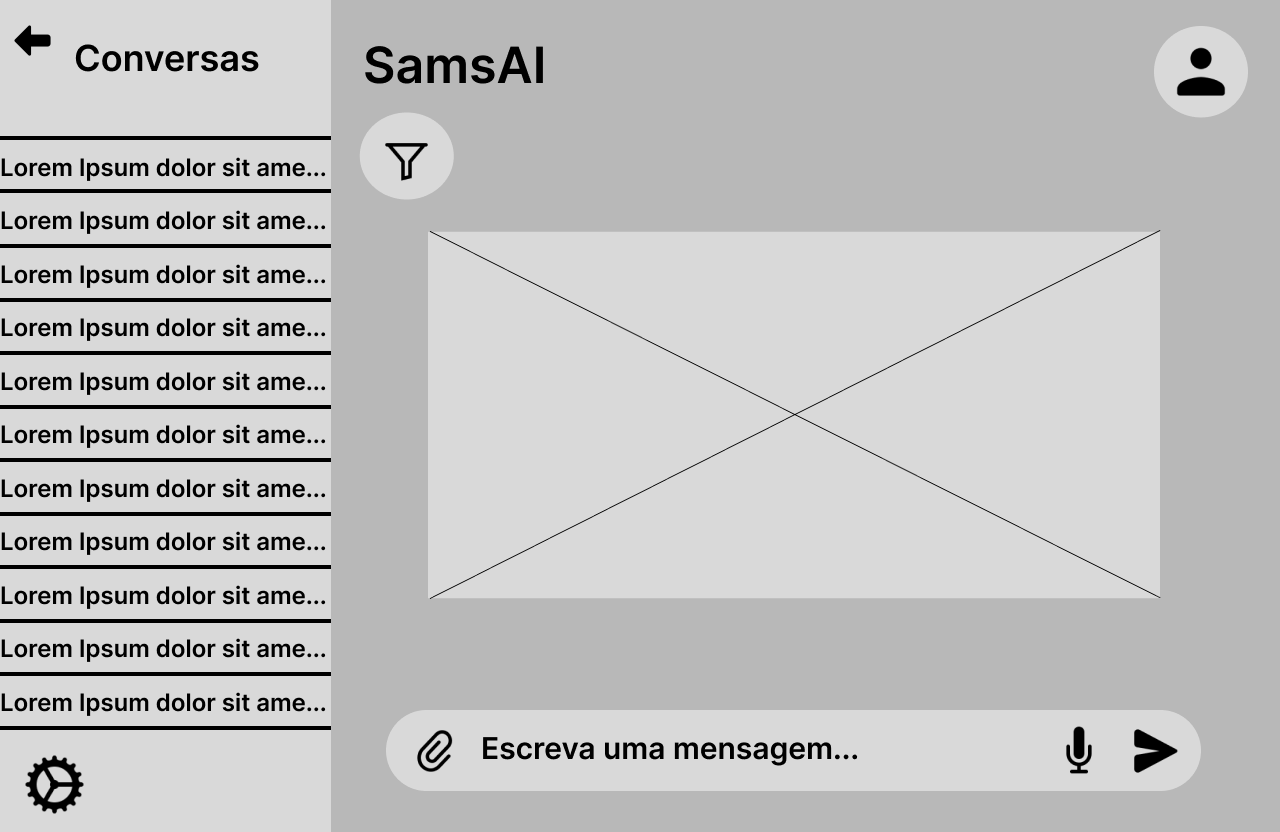
\includegraphics[width=0.8\linewidth]{Tela Inicial.png}
    \caption{Tela para iniciar uma conversa com o chatbot}
    \label{fig:enter-label}
\end{figure}

\section{Tela de conversa com a IA}
Assim que o usuário envia uma mensagem ao modelo, ele retorna uma resposta, que pode ser ouvida clicando-se no ícone do alto-falante.

\begin{figure}[h]
    \centering
    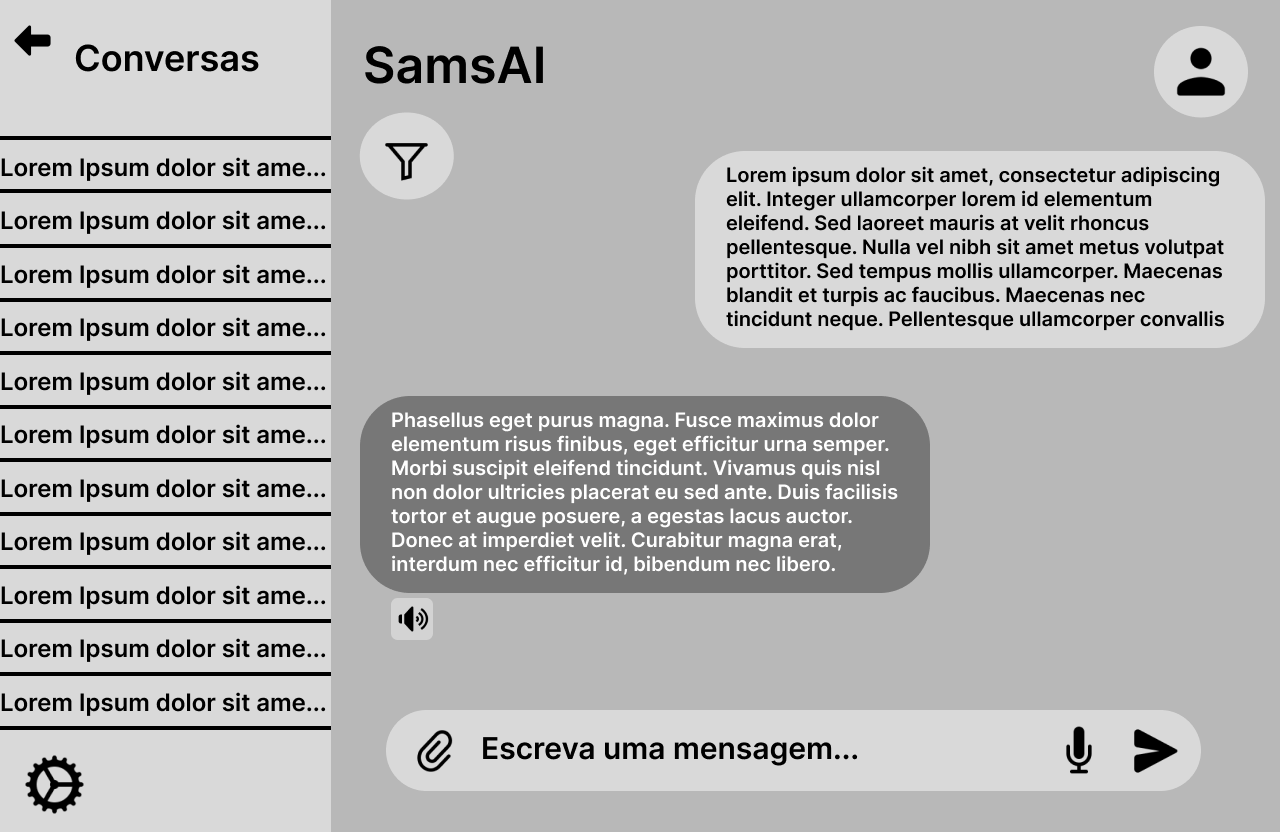
\includegraphics[width=0.8\linewidth]{Tela de Conversa com a IA.png}
    \caption{Tela exibindo a conversa entre o usuário e a IA}
    \label{fig:enter-label}
\end{figure}

\section{Tela com filtro para respostas}
Para obter respostas mais precisas, o usuário pode utilizar um filtro, clicando no ícone localizado no canto superior esquerdo. Nele, é possível filtrar os processos pelos: tipos documentos, os tipos de decisão, os tipos de processo, tribunais, estado, período, relator e advogado do caso.

\begin{figure}[h]
    \centering
    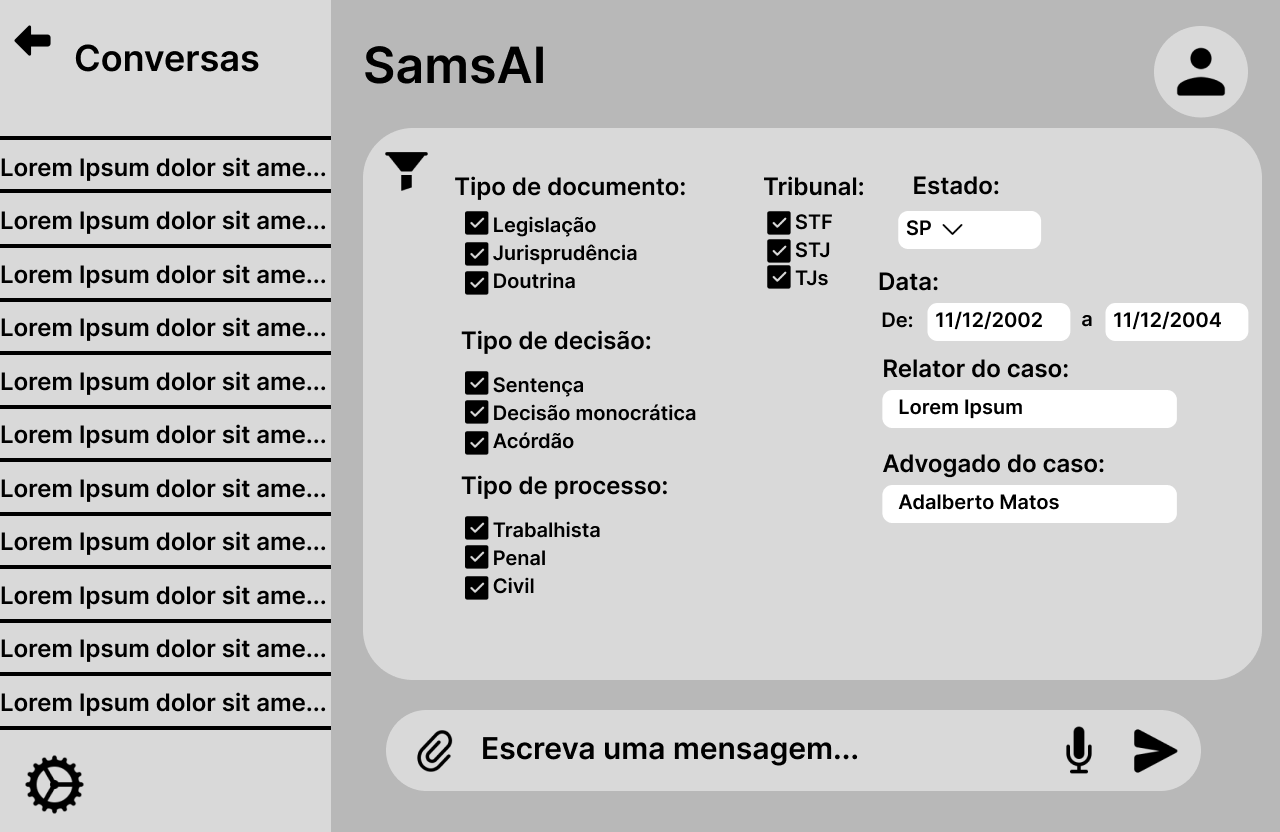
\includegraphics[width=0.8\linewidth]{Tela de Filtro.png}
    \caption{Tela exibindo as opções de filtragem para pesquisa}
    \label{fig:enter-label}
\end{figure}

\newpage
\section{Tela de configurações}
Caso o usuário sinta necessidade de configurar a aplicação, ele pode acessar as configurações pelo ícone no canto esquerdo inferior da tela. Nesta tela, ele será capaz de alternar o tema da aplicação entre claro e escuro, além de poder descrever

\begin{figure}[h!]
    \centering
    \includegraphics[width=0.8\linewidth]{Tela de configurações.png}
    \caption{Tela para o usuário configurar a interface e as respostas da IA}
    \label{fig:enter-label}
\end{figure}

\newpage
\section{Tela para dar feedback ou sair}
O usuário pode, a qualquer momento, fornecer um feedback sobre sua experiência com o SamsAI ou sair da aplicação clicando em sua imagem de perfil e escolhendo uma destas opções.

\begin{figure}[h!]
    \centering
    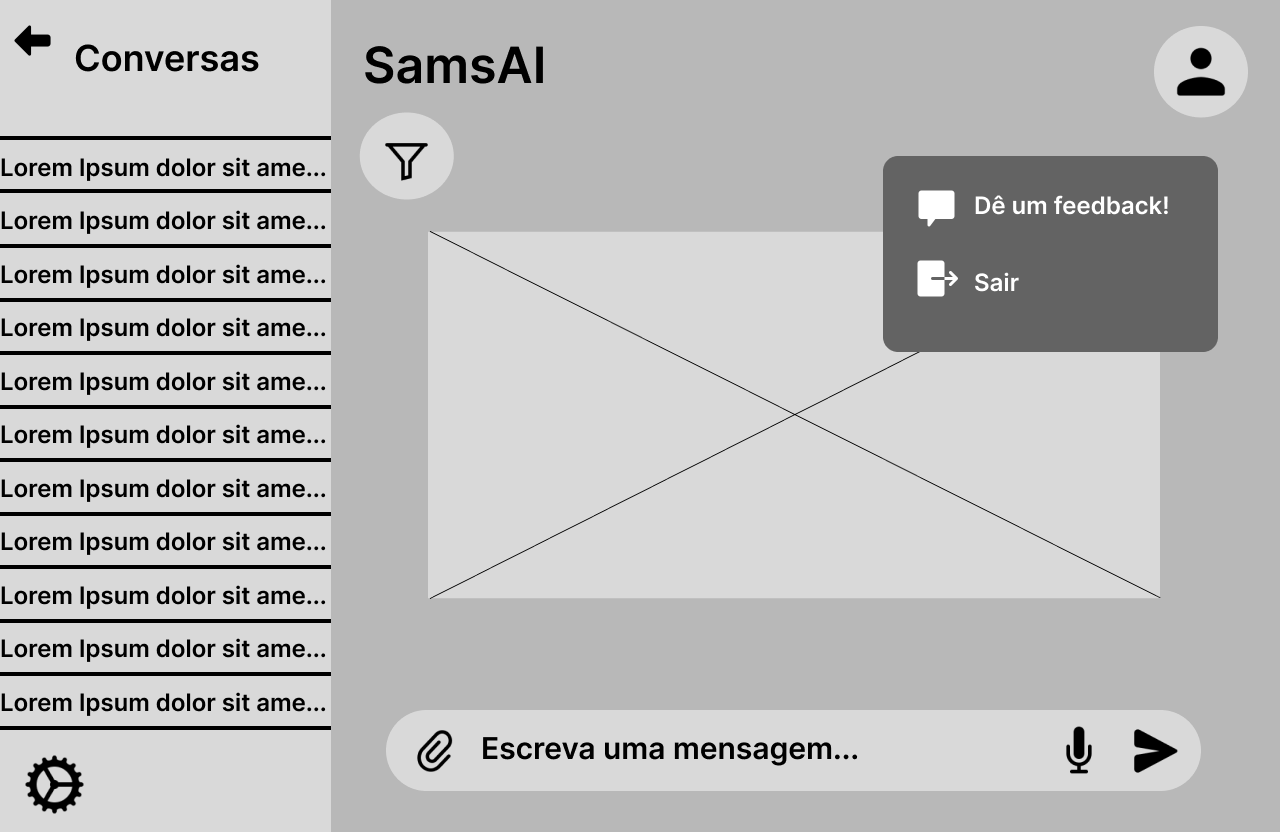
\includegraphics[width=0.8\linewidth]{Tela de feedback.png}
    \caption{Tela para dar um feedback ou sair da aplicação}
    \label{fig:enter-label}
\end{figure}



\chapter{MODELAGEM}
Neste capítulo, a fim de aprofundar a interpretação acerca do projeto, apresentaremos: diagrama de casos de uso, especificações dos principais casos de uso, diagrama de classes de domínio e, por fim, um diagrama de sequência baseado nos principais casos de uso.

\section{Diagrama de caso de uso}
Neste diagrama, apresentamos os casos de uso que podem ser feitos pelo único ator existente, o usuário.

\begin{figure}[h!]
    \centering
    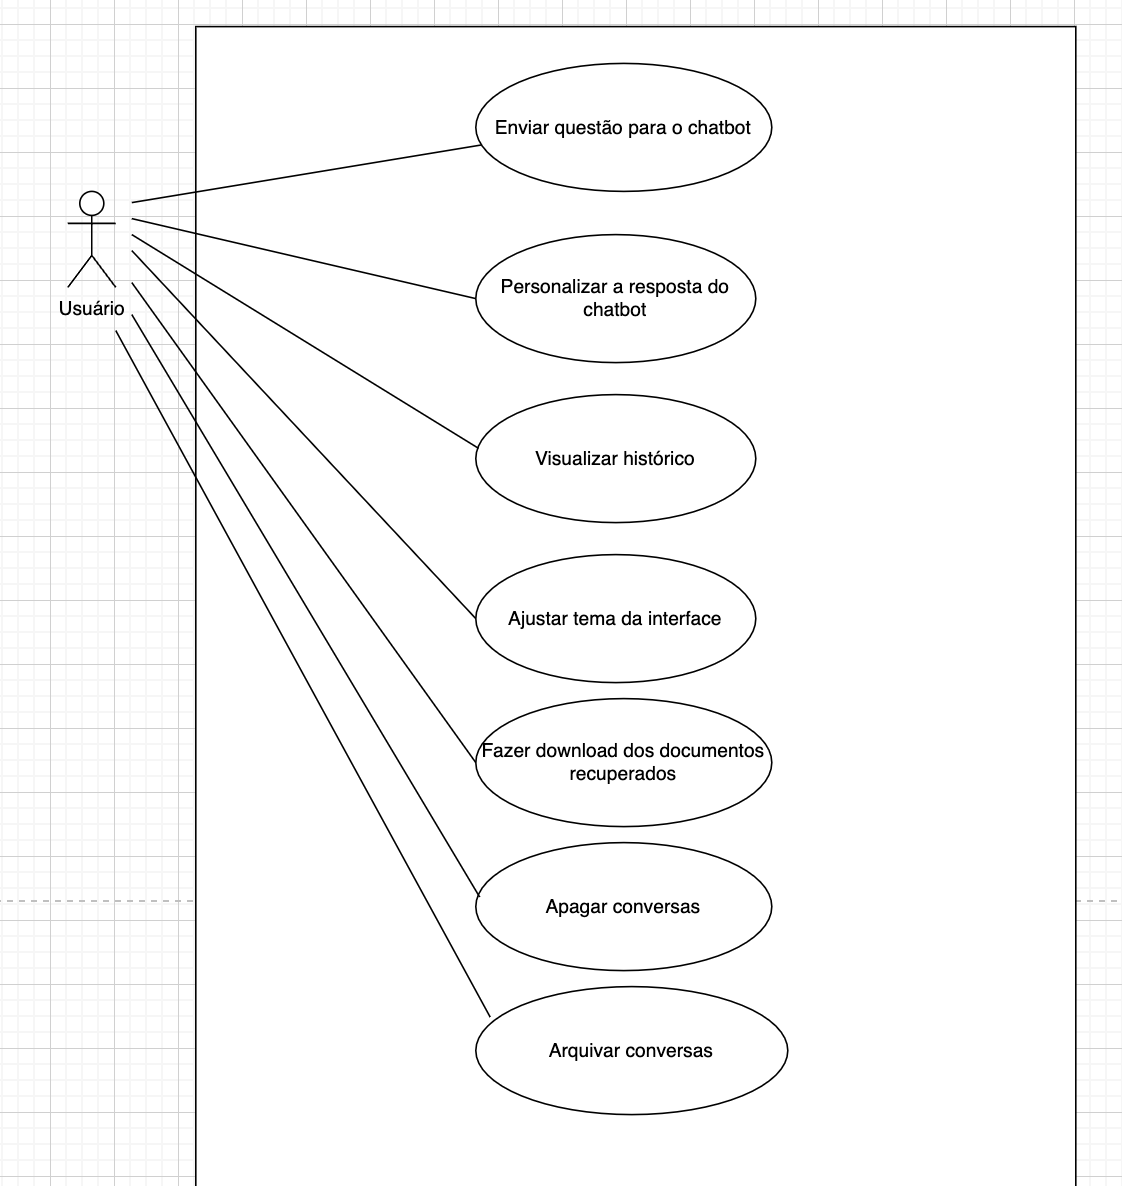
\includegraphics[width=0.8\linewidth]{Diagrama de casos de uso.png}
    \caption{Diagrama de casos de uso do projeto}
    \label{fig:enter-label}
\end{figure}

\section{Especificação dos principais casos de uso}
Nesta subseção, apresentaremos a especificação dos principais casos de uso do projeto: enviar questão para o chatbot, ajustar interface e apagar uma conversa.

\subsection{Enviar questão para o chatbot}
%--------------------- TABELA DE IDENTIFICAÇÃO DO UC001 ----------------------------------------------
\begin{table}[htb]

\ABNTEXfontereduzida
\caption[Tabela do caso de uso enviar questão para o chatbot]{Tabela do caso de uso enviar questão para o chatbot}
\label{tab-nivinv}
\hspace*{2.5cm}
\begin{tabular}{|>{\centering\arraybackslash}m{2.5cm}|>{\centering\arraybackslash}m{8cm}|}
  \hline
    Identificador & UC001  \\ \hline
    Nome & Enviar questão para o chatbot  \\ \hline
    Atores & Usuário  \\ \hline
    Sumário & O usuário envia uma questão ao sistema e este lhe responde com as informações solicitadas  \\ \hline
    Pré-condições & -  \\ \hline
    Pós-condições & Uma resposta é fornecida pelo sistema  \\ \hline
    Regras de Negócio & 1) O texto inserido pelo usuário pode ter no máximo 4000 caracteres. 
     
    2) A resposta deve ser baseada em documentos com pelo menos 50\% de proximidade. \\ \hline
    
    
\end{tabular}
\legend{Fonte: Próprios autores}
\end{table}
%--------------------- TABELA DE IDENTIFICAÇÃO DO UC001 ----------------------------------------------

%--------------------- TABELA DE FLUXO PRINCIPAL DO UC001 ----------------------------------------------
\begin{table}[htb]

\ABNTEXfontereduzida
\caption[Tabela de fluxo principal do UC001]{Tabela de fluxo principal do UC001}
\label{tab-nivinv}
\hspace*{1.5cm}
\begin{tabular}{|>{\centering\arraybackslash}m{6cm}|>{\centering\arraybackslash}m{6cm}|}
  \hline
  \multicolumn{2}{|>{\centering\arraybackslash}m{12cm}|}{\textbf{Fluxo Principal}} \\ \hline
    Ações do ator & Ações do sistema  \\ \hline
    1) O usuário digita e envia um texto pelo prompt. & 2) O texto aparece no chat, o prompt é bloqueado e o sistema gera uma notificação que a resposta está sendo gerada.  \\ \hline
      & 3) O sistema faz a conversão da entrada de texto para uma representação numérica e consulta dados próximos da fonte externa.  \\ \hline
      & 4) O sistema retorna os dados com maior proximidade e aplica no LLM.  \\ \hline
      & 5) Com base nos dados recebidos, o LLM gera uma resposta embaixo do texto de entrada.  \\ \hline
      & 6) O sistema indica a disponibilidade para uma nova questão. \\ \hline
    
\end{tabular}
\legend{Fonte: Próprios autores}
\end{table}
%--------------------- TABELA DE FLUXO PRINCIPAL DO UC001 ----------------------------------------------

%--------------------- TABELA DE FLUXO ALTERNATIVO NO PASSO 2 DO UC001 ----------------------------------------------
\begin{table}[htb]

\ABNTEXfontereduzida
\caption[Tabela de fluxo alternativo no passo 2 do UC001]{Tabela de fluxo alternativo no passo 2 do UC001}
\label{tab-nivinv}
\hspace*{1.5cm}
\begin{tabular}{|>{\centering\arraybackslash}m{6cm}|>{\centering\arraybackslash}m{6cm}|}
  \hline
  \multicolumn{2}{|>{\centering\arraybackslash}m{12cm}|}{\textbf{Fluxo alternativo - Passo 2: O usuário quer interromper a geração de resposta}} \\ \hline
    Ações do ator & Ações do sistema  \\ \hline
    1) Entre os passos 1 e 6, o usuário clica na notificação para “parar de responder”. & 2) O sistema interrompe o processo de geração de resposta.  \\ \hline
      & 3) O sistema indica a disponibilidade para uma nova questão.  \\ \hline
\end{tabular}
\legend{Fonte: Próprios autores}
\end{table}
%--------------------- TABELA DE FLUXO ALTERNATIVO NO PASSO 2 DO UC001 ----------------------------------------------

%--------------------- TABELA DE FLUXO DE EXCEÇÃO NO PASSO 1 DO UC001 ----------------------------------------------
\begin{table}[htb]

\ABNTEXfontereduzida
\caption[Tabela de fluxo de exceção no passo 1 do UC001]{Tabela de fluxo de exceção no passo 1 do UC001}
\label{tab-nivinv}
\hspace*{1.5cm}
\begin{tabular}{|>{\centering\arraybackslash}m{6cm}|>{\centering\arraybackslash}m{6cm}|}
  \hline
  \multicolumn{2}{|>{\centering\arraybackslash}m{12cm}|}{\textbf{Fluxo de exceção - Passo 1: Quantidade máxima de caracteres no prompt atingida}} \\ \hline
    Ações do ator & Ações do sistema  \\ \hline
    1) No passo 1, o usuário insere mais de 4000 caracteres no prompt & 2) O sistema indica que a quantidade máxima de caracteres no prompt foi atingida e limita o texto até 4000 caracteres  \\ \hline
\end{tabular}
\legend{Fonte: Próprios autores}
\end{table}
%--------------------- TABELA DE FLUXO DE EXCEÇÃO NO PASSO 1 DO UC001 ----------------------------------------------

%--------------------- TABELA DE FLUXO DE EXCEÇÃO NO PASSO 3 DO UC001 ----------------------------------------------
\begin{table}[htb]

\ABNTEXfontereduzida
\caption[Tabela de fluxo de exceção no passo 3 do UC001]{Tabela de fluxo de exceção no passo 3 do UC001}
\label{tab-nivinv}
\hspace*{1.5cm}
\begin{tabular}{|>{\centering\arraybackslash}m{6cm}|>{\centering\arraybackslash}m{6cm}|}
  \hline
  \multicolumn{2}{|>{\centering\arraybackslash}m{12cm}|}{\textbf{Fluxo de exceção - Passo 3: Não há dados com pelo menos 50\% de proximidade}} \\ \hline
    Ações do ator & Ações do sistema  \\ \hline
     1) No passo 1, o usuário insere um texto & 2) O sistema não encontra dados com pelo menos 50\% de proximidade com o texto de entrada  \\ \hline
      & 3) O sistema instrui ao LLM gerar uma resposta de “informações não encontradas”.  \\ \hline
      & 4) O LLM gera a resposta embaixo do texto de entrada.  \\ \hline
      & 5) O sistema indica a disponibilidade para uma nova questão.  \\ \hline
\end{tabular}
\legend{Fonte: Próprios autores}
\end{table}
%--------------------- TABELA DE FLUXO DE EXCEÇÃO NO PASSO 3 DO UC001 ----------------------------------------------
\clearpage
\subsection{Ajustar tema da interface}

%--------------------- TABELA DE IDENTIFICAÇÃO DO UC002 ----------------------------------------------
\begin{table}[htb]

\ABNTEXfontereduzida
\caption[Tabela do caso de uso ajustar tema da interface]{Tabela do caso de uso ajustar tema da interface}
\label{tab-nivinv}
\hspace*{2cm}
\begin{tabular}{|>{\centering\arraybackslash}m{2.5cm}|>{\centering\arraybackslash}m{8cm}|}
  \hline
    Identificador & UC002  \\ \hline
    Nome & Ajustar tema da interface  \\ \hline
    Atores & Usuário  \\ \hline
    Sumário & O usuário altera o tema da interface de escuro para claro ou de claro para escuro \\ \hline
    Pré-condições & -  \\ \hline
    Pós-condições & O tema da interface se torna aquele definido pelo usuário \\ \hline
    Regras de Negócio & 1) Os dois únicos temas disponíveis para a interface são o claro e escuro \\ \hline   
\end{tabular}
\legend{Fonte: Próprios autores}
\end{table}
%--------------------- TABELA DE IDENTIFICAÇÃO DO UC002 ----------------------------------------------

%--------------------- TABELA DE FLUXO PRINCIPAL DO UC002 ----------------------------------------------
\begin{table}[htb]

\ABNTEXfontereduzida
\caption[Tabela de fluxo principal do UC002]{Tabela de fluxo principal do UC002}
\label{tab-nivinv}
\hspace*{1.5cm}
\begin{tabular}{|>{\centering\arraybackslash}m{6cm}|>{\centering\arraybackslash}m{6cm}|}
  \hline
  \multicolumn{2}{|>{\centering\arraybackslash}m{12cm}|}{\textbf{Fluxo Principal}} \\ \hline
    Ações do ator & Ações do sistema  \\ \hline
    1) Usuário clica no ícone de configurações & 2) Sistema exibe a tela de configurações  \\ \hline
     3) Usuário muda o tema da interface para o tema desejado  & 4) Sistema adota o novo tema escolhido \\ \hline
\end{tabular}
\legend{Fonte: Próprios autores}
\end{table}
%--------------------- TABELA DE FLUXO PRINCIPAL DO UC002 ----------------------------------------------

%--------------------- TABELA DE FLUXO ALTERNATIVO NO PASSO 2 DO UC002 ----------------------------------------------
\begin{table}[htb]

\ABNTEXfontereduzida
\caption[Tabela de fluxo alternativo no passo 2 do UC002]{Tabela de fluxo alternativo no passo 2 do UC002}
\label{tab-nivinv}
\hspace*{1.5cm}
\begin{tabular}{|>{\centering\arraybackslash}m{6cm}|>{\centering\arraybackslash}m{6cm}|}
  \hline
  \multicolumn{2}{|>{\centering\arraybackslash}m{12cm}|}{\textbf{Fluxo alternativo - Passo 2: O usuário desiste de trocar o tema}} \\ \hline
    Ações do ator & Ações do sistema  \\ \hline
    1) No passo 2, o usuário sai das configurações clicando no X no canto superior direito & 2) Sistema retorna à tela com a conversa em que se encontrava  \\ \hline
\end{tabular}
\legend{Fonte: Próprios autores}
\end{table}
%--------------------- TABELA DE FLUXO ALTERNATIVO NO PASSO 2 DO UC002 ----------------------------------------------
\clearpage
\subsection{Apagar uma conversa}
%--------------------- TABELA DE IDENTIFICAÇÃO DO UC003 ----------------------------------------------
\begin{table}[htb]

\ABNTEXfontereduzida
\caption[Tabela do caso de uso apagar uma conversa]{Tabela do caso de uso apagar uma conversa}
\label{tab-nivinv}
\hspace*{2cm}
\begin{tabular}{|>{\centering\arraybackslash}m{2.5cm}|>{\centering\arraybackslash}m{8cm}|}
  \hline
    Identificador & UC003  \\ \hline
    Nome & Apagar uma conversa \\ \hline
    Atores & Usuário  \\ \hline
    Sumário & O usuário apaga uma conversa do sistema que considera inútil \\ \hline
    Pré-condições & O usuário deve estar logado na aplicação  \\ \hline
    Pós-condições & A conversa deve estar excluída do banco de dados com as conversas daquele usuário \\ \hline
    Regras de Negócio & 1) Todas as conversas dos usuários devem ser armazenadas num banco de dados
    
    2) O usuário deve ser capaz de apagar ou arquivar qualquer conversa a qualquer momento\\ \hline   
\end{tabular}
\legend{Fonte: Próprios autores}
\end{table}
%--------------------- TABELA DE IDENTIFICAÇÃO DO UC003 ----------------------------------------------

%--------------------- TABELA DE FLUXO PRINCIPAL DO UC003 ----------------------------------------------
\begin{table}[htb]

\ABNTEXfontereduzida
\caption[Tabela de fluxo principal do UC003]{Tabela de fluxo principal do UC003}
\label{tab-nivinv}
\hspace*{1.5cm}
\begin{tabular}{|>{\centering\arraybackslash}m{6cm}|>{\centering\arraybackslash}m{6cm}|}
  \hline
  \multicolumn{2}{|>{\centering\arraybackslash}m{12cm}|}{\textbf{Fluxo Principal}} \\ \hline
    Ações do ator & Ações do sistema  \\ \hline
    1) Usuário visualiza o histórico de conversas e escolhe uma das conversas para deletar &    \\ \hline
    2) Usuário passa o mouse sobre conversa  & 3) Sistema exibe ícone de mais opções ao lado do nome da conversa \\ \hline
    4) Usuário clica sobre o ícone de opções  & 5) Sistema exibe opções de: Renomear, Arquivar ou Excluir uma conversa \\ \hline
    6) Usuário escolhe opção de Excluir & 7) Sistema pergunta se o usuário tem certeza de que deseja excluir aquela conversa\\ \hline
    8) Usuário confirma que sim clicando em "Excluir" & 9) Sistema exclui conversa de seu banco de dados\\ \hline
\end{tabular}
\legend{Fonte: Próprios autores}
\end{table}
%--------------------- TABELA DE FLUXO PRINCIPAL DO UC003 ----------------------------------------------

%--------------------- TABELA DE FLUXO ALTERNATIVO NO PASSO 6 DO UC003 ----------------------------------------------
\begin{table}[htb]

\ABNTEXfontereduzida
\caption[Tabela de fluxo alternativo no passo 6 do UC003]{Tabela de fluxo alternativo no passo 6 do UC003}
\label{tab-nivinv}
\hspace*{1.5cm}
\begin{tabular}{|>{\centering\arraybackslash}m{6cm}|>{\centering\arraybackslash}m{6cm}|}
  \hline
  \multicolumn{2}{|>{\centering\arraybackslash}m{12cm}|}{\textbf{Fluxo alternativo - Passo 6: O usuário desiste de excluir a mensagem
}} \\ \hline
    Ações do ator & Ações do sistema  \\ \hline
    1) No passo 6, o usuário desiste de clicar sobre o botão excluir &   \\ \hline
\end{tabular}
\legend{Fonte: Próprios autores}
\end{table}
%--------------------- TABELA DE FLUXO ALTERNATIVO NO PASSO 6 DO UC003 ----------------------------------------------

%--------------------- TABELA DE FLUXO ALTERNATIVO NO PASSO 8 DO UC003 ----------------------------------------------
\begin{table}[htb]

\ABNTEXfontereduzida
\caption[Tabela de fluxo alternativo no passo 8 do UC003]{Tabela de fluxo alternativo no passo 8 do UC003}
\label{tab-nivinv}
\hspace*{1.5cm}
\begin{tabular}{|>{\centering\arraybackslash}m{6cm}|>{\centering\arraybackslash}m{6cm}|}
  \hline
  \multicolumn{2}{|>{\centering\arraybackslash}m{12cm}|}{\textbf{Fluxo alternativo - Passo 6: O usuário desiste de excluir a conversa}} \\ \hline
    Ações do ator & Ações do sistema  \\ \hline
    1) No passo 6, o usuário desiste de clicar sobre o botão excluir &   \\ \hline
\end{tabular}
\legend{Fonte: Próprios autores}
\end{table}
%--------------------- TABELA DE FLUXO ALTERNATIVO NO PASSO 8 DO UC003 ----------------------------------------------
\clearpage
\section{Diagrama de classes de domínio}
Nesta seção, exibimos a seguir o diagrama de classes de domínio contendo as classes identificadas no projeto (Usuário, Requisição, Modelo de IA, Codificador, Documento e Banco de Dados) e as relações entre elas.

\begin{figure}[h]
    \centering
    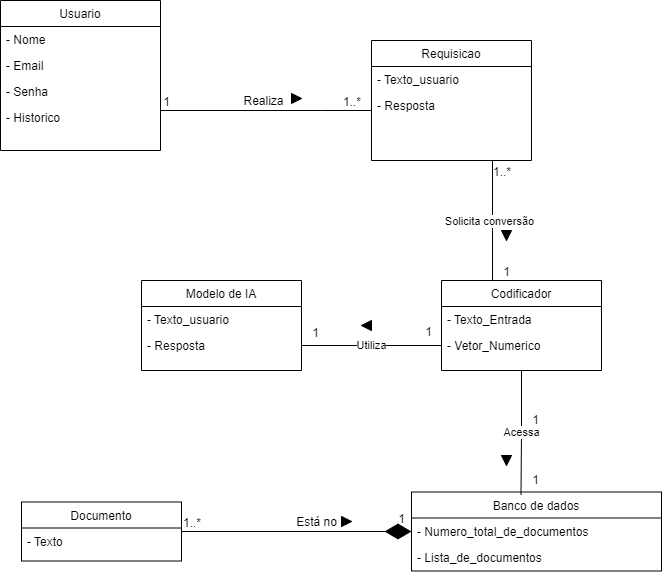
\includegraphics[width=0.8\linewidth]{Diagrama classes.drawio (1).png}
    \caption{Diagrama de classes de domínio}
    \label{fig:enter-label}
\end{figure}

\clearpage
\section{Diagrama de sequência}
Nesta seção, exibimos a seguir o diagrama de sequência do caso de uso principal, enviar questão para o chatbot.

\begin{figure}[h]
    \centering
    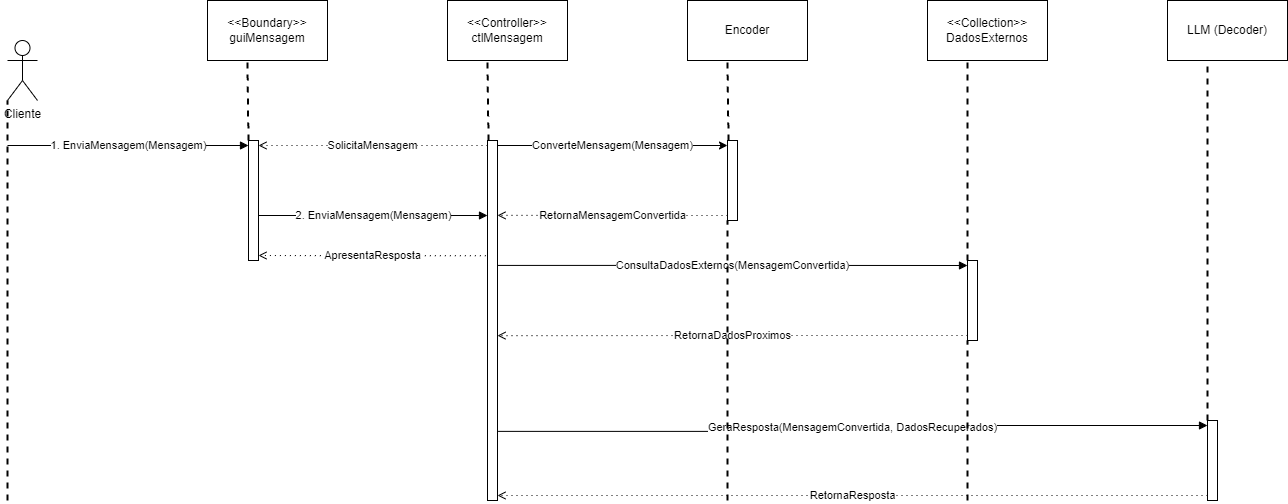
\includegraphics[width=1\linewidth]{DiagramaSequencia.drawio.png}
    \caption{Diagrama de sequência do caso de uso enviar questão para o chatbot}
    \label{fig:enter-label}
\end{figure}

\chapter{DESCRIÇÃO DA ARQUITETURA}
%Breve descrição...

\section{Arquitetura em camadas}

\begin{figure}[h]
    \centering
    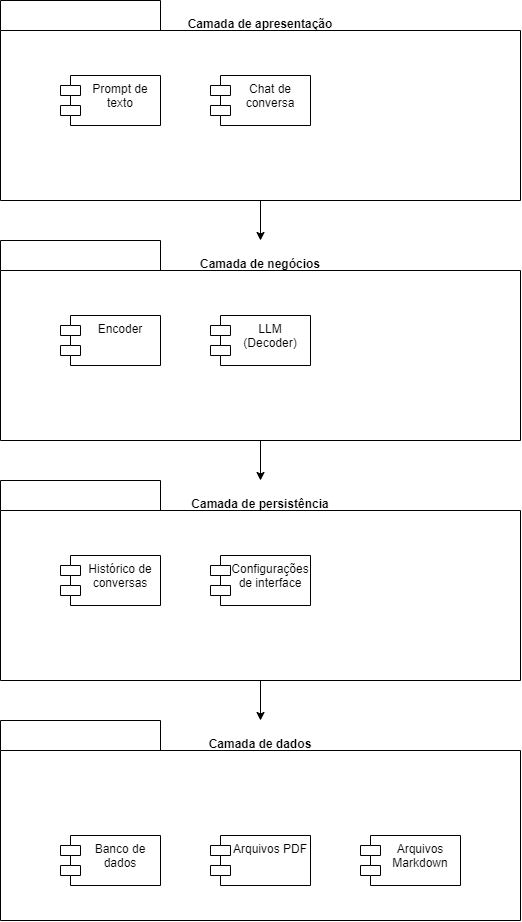
\includegraphics[width=0.5\linewidth]{ArquiteturaCamadas.drawio.png}
    \caption{Diagrama UML da arquitetura em camadas}
    \label{fig:enter-label}
\end{figure}

\clearpage
\section{Pipeline}

\begin{figure}[h]
    \centering
    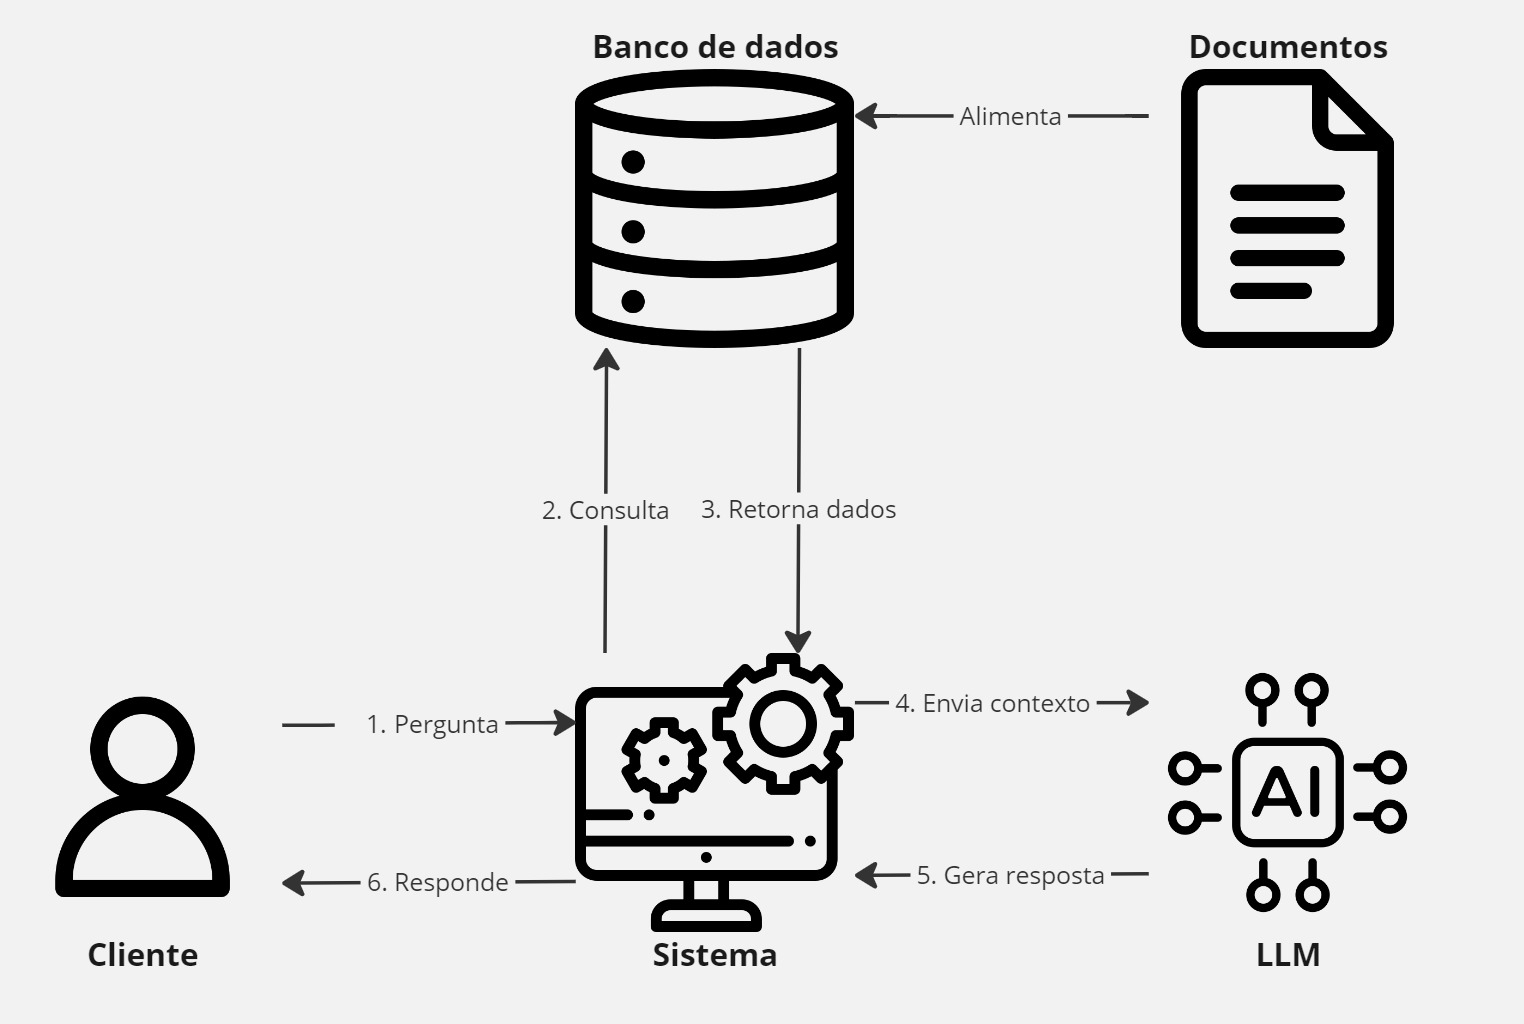
\includegraphics[width=0.8\linewidth]{Pipeline.jpg}
    \caption{Pipeline}
    \label{fig:enter-label}
\end{figure}

\section{Linguagens de Programação}
A ideia de nosso projeto é construir o sistema em Python por meio do uso de frameworks adequados para desenvolvimento de aplicações com LLMs.Também será usado HTML/CSS e Javascript para construir a estrutura da interface da aplicação. Além disso, o Javascript também será usado para integrar a interface com o sistema.


\section{Frameworks}
    \subsection{LangChain}
    O LangChain é um framework para desenvolvimento de aplicações que utilizam LLMs. Ele pode ser usado para criar chatbots e agentes virtuais personalizados, analisar grandes volumes de texto para extração de informação e integração com diversas APIs.

    \subsection{LangGraph}
    Já o LangGraph é uma extensão do LangChain focada para a construção de aplicações mais robustas com multi-agentes. Sua biblioteca permite a criação de sistemas complexos com vários agentes que interagem entre si, cada um executando tarefas específicas e trocando informações conforme necessário. Além disso, oferece gerenciamento automático de estado, permitindo rastrear e manter informações ao longo de várias interações, garantindo que o sistema mantenha o contexto e responda adequadamente a novas entradas.

    \subsection{LlamaIndex}
    O LlamaIndex é um framework para conectar fontes de dados personalizadas a LLMs. Sua biblioteca oferece ferramentas para ingerir, estruturar e consultar dados de fontes estruturadas e não-estruturadas para a aplicações com LLMs.
    
%------------------------------FAZER TUDO ATÉ AQUI------------------------------------

\end{document}

